%=================================================================
\section{\DIFdelbegin \DIFdel{Introduction}\DIFdelend \DIFaddbegin \DIFadd{Problem Definition}\DIFaddend }\label{sec-intro}
\DIFdelbegin %DIFDELCMD < 

%DIFDELCMD < %%%
\DIFdelend %\todo{Narrow down to a topic; Dig a hole; Fill the hole}
\DIFdelbegin %DIFDELCMD < \todo{Formula for Introduction}
%DIFDELCMD < %%%
\DIFdelend \DIFaddbegin \DIFadd{The source of data for forecasting traffic flows in metropolitan areas in the USA is mainly based on kaggle competitions. The data contains characteristics such as time, coordinates, direction, etc. The aim of the article is to predict the amount of congestion at a particular time.}\par 
\DIFadd{The files and data attrubitions are described in Table 1:
}\begin{center}
	\begin{table}[htbp]
		\setlength{\abovecaptionskip}{2pt}
		\centering
		\caption{\DIFaddFL{DATA}}
		\begin{tabular}{ c | c | c }
			\toprule
			%DIF >  after \\: \hline or \cline{col1-col2} \cline{col3-col4} ...
			\DIFaddFL{File    }&\DIFaddFL{Description      }& \DIFaddFL{Attribution       }\\
			\midrule
			\DIFaddFL{train.csv       }&  \makecell{traffic congestion from April\\through September of 1991}   &  \makecell{row_id,time,x,y,\\direction,congestion}       \\
			\midrule
			\DIFaddFL{test.csv       }& \makecell{hourly predictions \\on the day of 1991-09-30}   &\makecell{row_id,time,x,y,\\direction}     \\
			\bottomrule
		\end{tabular}
	\end{table}
\end{center}
\DIFaddend 



%\gangli{``narrow in on topic'' reminds you 
%that readers and reviewers only know that this is a AI or HTM research paper (and maybe have read the title/abstract). 
%You need to help them figure out what topic and area of research paper this is. 
%You _don't_ need to wax poetic about the topic's importance.}

%\gangli{`dig a hole'' reminds you that 
%you need to convince the reader that there's a problem with the state of the world. 
%Prior work may exist but it's either missing something important or there's a missing opportunity. 
%The reader should be drooling for a bright future just out of reach.}

%\gangli{``fill the hole'' reminds you to show the reader 
%how and why the paper they're reading will fix these problems and deliver us into a better place. 
%You don't need a whirlwind summary of the technical details, 
%but you need readers convinced (and in a good mood) to keep reading.}

\DIFdelbegin %DIFDELCMD < \gangli{A good paper introduction is fairly formulaic. 
%DIFDELCMD < If you follow a simple set of rules, 
%DIFDELCMD < you can write a very good introduction. 
%DIFDELCMD < The following outline can be varied. 
%DIFDELCMD < For example, 
%DIFDELCMD < you can use two paragraphs instead of one, 
%DIFDELCMD < or you can place more emphasis on one aspect of the intro than another. 
%DIFDELCMD < But in all cases, 
%DIFDELCMD < all of the points below need to be covered in an introduction, 
%DIFDELCMD < and in most papers, 
%DIFDELCMD < you don't need to cover anything more in an introduction.}
%DIFDELCMD < 

%DIFDELCMD < %%%
\DIFdelend %\todo{The importance of the area}
%\blindtext
\DIFdelbegin %DIFDELCMD < \todo{Motivation}
%DIFDELCMD < %%%
\DIFdel{At a high level, 
what is the problem area you are working in and why is it important? 
It is important to set the larger context here. 
Why is the problem of interest and importance to the larger community?
}\DIFdelend 


%DIF < \todo{The problems faced by most current methods}
%DIF < \blindtext
\DIFdelbegin %DIFDELCMD < \todo{What is the specific problem considered in this paper?}
%DIFDELCMD < %%%
\DIFdel{This paragraph narrows down the topic area of the paper. 
In the first paragraph you have established general context and importance.Here you establish specific context and background.
}%DIFDELCMD < 

%DIFDELCMD < %%%
%DIF < \todo{What can be addressed by existing methods; Why those problems are challenges to existing methods?}
%DIF < \blindtext
%DIFDELCMD < \todo{Contribution}
%DIFDELCMD < %%%
\DIFdel{"In this paper, we show that ...". 
This is the key paragraph in the intro - you summarize, in one paragraph, what are the main contributions of your paper given the context 
you have established in paragraphs 1 and 2. 
What isthe general approach taken? 
Why are the specific results significant? 
This paragraph must be really good. 
}%DIFDELCMD < 

%DIFDELCMD < %%%
\DIFdel{You should think about how to structure these one or 
two paragraph summaries of what your paper is all about. 
If there are two or three main results, then you might consider itemizing them with bullets or in test. 
}\DIFdelend \DIFaddbegin \section{\DIFadd{Data Processing}} \label{sec-dataprocess}
\DIFadd{Since the training data has both segmentable and mergeable data, we segmented the temporal data and merged the x, y and direction data.}\par
\DIFadd{First, we divide the 24 hours into 6 time periods, as in Table 2:
}\begin{center}
	\begin{table}[htbp]
		\setlength{\abovecaptionskip}{2pt}
		\caption{\DIFaddFL{period}}
		\begin{tabular}{ c | c | c | c }
			\toprule
			\DIFaddFL{period    }&\DIFaddFL{Description   }&  \DIFaddFL{period    }&\DIFaddFL{Description      }\\
			\midrule
			\DIFaddFL{Late Night     }& \DIFaddFL{0:00-4:00 }& \DIFaddFL{Noon     }& \DIFaddFL{12:00-16:00 }\\
			\midrule
			\DIFaddFL{Early Morning     }& \DIFaddFL{4:00-8:00 }& \DIFaddFL{Evening     }& \DIFaddFL{16:00-20:00 }\\
			\midrule
			\DIFaddFL{Morning     }& \DIFaddFL{8:00-12:00 }&  \DIFaddFL{Night     }& \DIFaddFL{20:00-24:00 }\\
			\bottomrule
		\end{tabular}
	\end{table}
\end{center}\par
\DIFadd{Second, we split the time into the following features:
}\DIFaddend \begin{itemize}
	\DIFaddbegin \setlength{\itemsep}{-0.9ex} 
	\DIFaddend \item
	\DIFdelbegin \DIFdel{e.g., First ...
	}\DIFdelend \DIFaddbegin \smallskip  
	\DIFadd{month
	}\DIFaddend \item
	\DIFdelbegin \DIFdel{e.g., Second . ..
	}\DIFdelend \DIFaddbegin \smallskip
	\DIFadd{weekday
	}\DIFaddend \item
	\DIFdelbegin \DIFdel{e.g., Third ...
}\DIFdelend \DIFaddbegin \smallskip
	\DIFadd{minute
	}\item
	\smallskip
	\DIFadd{is_month_start
	}\item
	\smallskip
	\DIFadd{is_month_end
	}\item
	\smallskip
	\DIFadd{is_weekday
	}\item
	\smallskip
	\DIFadd{is_Monday
	}\item
	\smallskip
	\DIFadd{is_Friday
	}\item
	\smallskip
	\DIFadd{period
	}\item
	\smallskip
	\DIFadd{road:x+y+direction(00EB)
}\DIFaddend \end{itemize}
\DIFdelbegin \DIFdel{If the results fall broadly into two categories, you can bring out that distinction here.For example, "Our results are both theoretical and applied in nature.(two sentences follow, one each on theory and application)
"
}\DIFdelend 



%DIF < \todo{What provides the motivation of this work? What are the research issues? What is the rationale of this work? }
%DIF < \blindtext
\DIFdelbegin %DIFDELCMD < \todo{At a high level what are the differences in what you are doing, and what others have done? }
%DIFDELCMD < %%%
\DIFdel{Keep this at a high level, you can refer to a future section where specific details and differences will be given.
	But it is important for the reader to know at a high level, what is new about this work compared to other work in the area.
}%DIFDELCMD < 

%DIFDELCMD < %%%
%DIF < \todo{What we have done and what are the contributions.}
%DIF < \blindtext
%DIFDELCMD < \todo{A roadmap for the rest of the paper}
%DIFDELCMD < %%%
\DIFdel{"The remainder of this paper is structured as follows..." 
Give the reader a roadmap for the rest of the paper.Avoid redundant phrasing, "In Section 2, In section 3, ... In Section 4, ... " }\DIFdelend \DIFaddbegin \section{\DIFadd{Data Description}} \label{datadescription}
\DIFadd{After the data has been processed, the data is explored for congestion, time, road, }\DIFaddend etc. \DIFaddbegin \DIFadd{to find more potential relationships between them.}\par
\DIFadd{Firstly, the histogram(figure 1) shows the congestion data, which is normalised as can be seen from the graph.}\par
\DIFadd{Secondly, we use various graphs to show the relationship between features and congestion.(fig.2-fig.9)
}\begin{figure}
	\setlength{\abovecaptionskip}{-0.1cm} 
	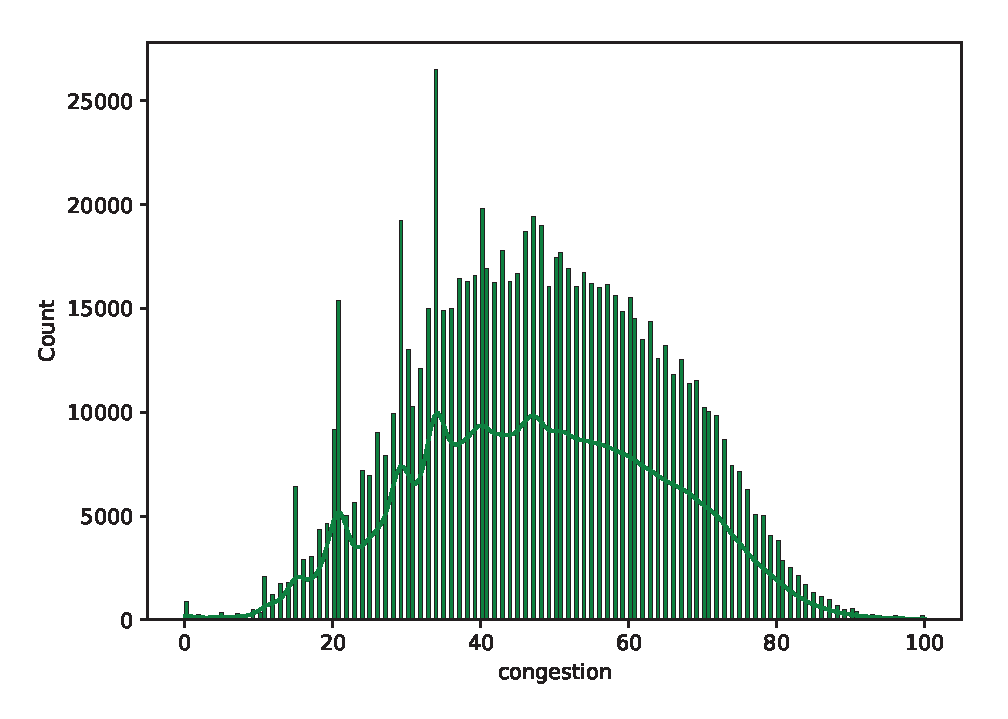
\includegraphics[width=10cm]{figure/congestion.eps}\\	
	\caption{\DIFaddFL{Congestion data}}
	\label{Congestion data}
\end{figure}
\DIFaddend 

\DIFdelbegin %DIFDELCMD < \gangli{A few general tips:
%DIFDELCMD < Don't spend a lot of time into the introduction 
%DIFDELCMD < telling the reader about what you don't do in the paper. 
%DIFDELCMD < Be clear about what you do do.
%DIFDELCMD < Does each paragraph have a theme sentence that sets the stage for the entire paragraph? Are the sentences and topics in the paragraph all related to each other?}
%DIFDELCMD < %%%
\DIFdelend \DIFaddbegin \begin{center}
	\begin{figure}[h]
		\setlength{\abovecaptionskip}{-0.1cm} 
		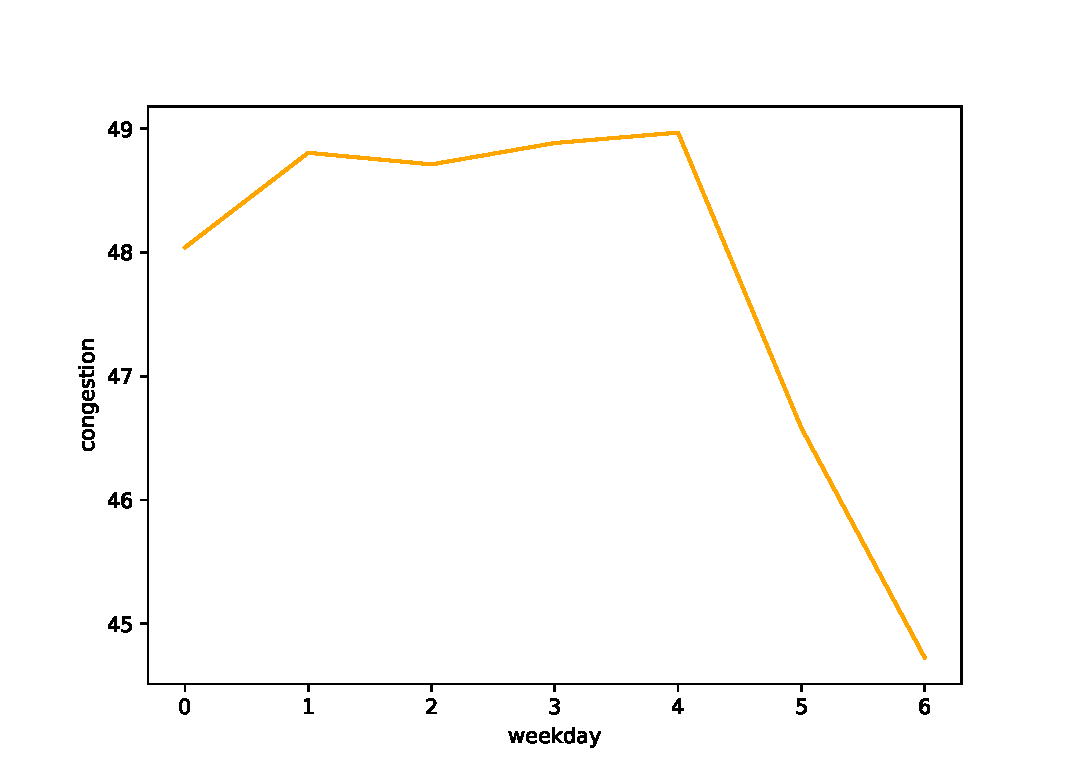
\includegraphics[width=10cm]{figure/weekday.eps}\\	
		\caption{\DIFaddFL{The effect of weekday on congestion}}
		\label{weekday}
	\end{figure}
\end{center}
\DIFaddend 

\DIFdelbegin %DIFDELCMD < \gangli{Does each paragraph have a theme 
%DIFDELCMD < sentence that sets the stage for the entire paragraph? 
%DIFDELCMD < Are the sentences and topics in the paragraph all related to each other?}
%DIFDELCMD < %%%
\DIFdelend \DIFaddbegin \begin{center}
	\DIFaddend 

	\DIFdelbegin %DIFDELCMD < \gangli{Do all of your tenses match up in a paragraph?}
%DIFDELCMD < %%%
\DIFdelend \DIFaddbegin \begin{figure}[htp]
	\setlength{\abovecaptionskip}{0.1cm} 
	\raggedleft
	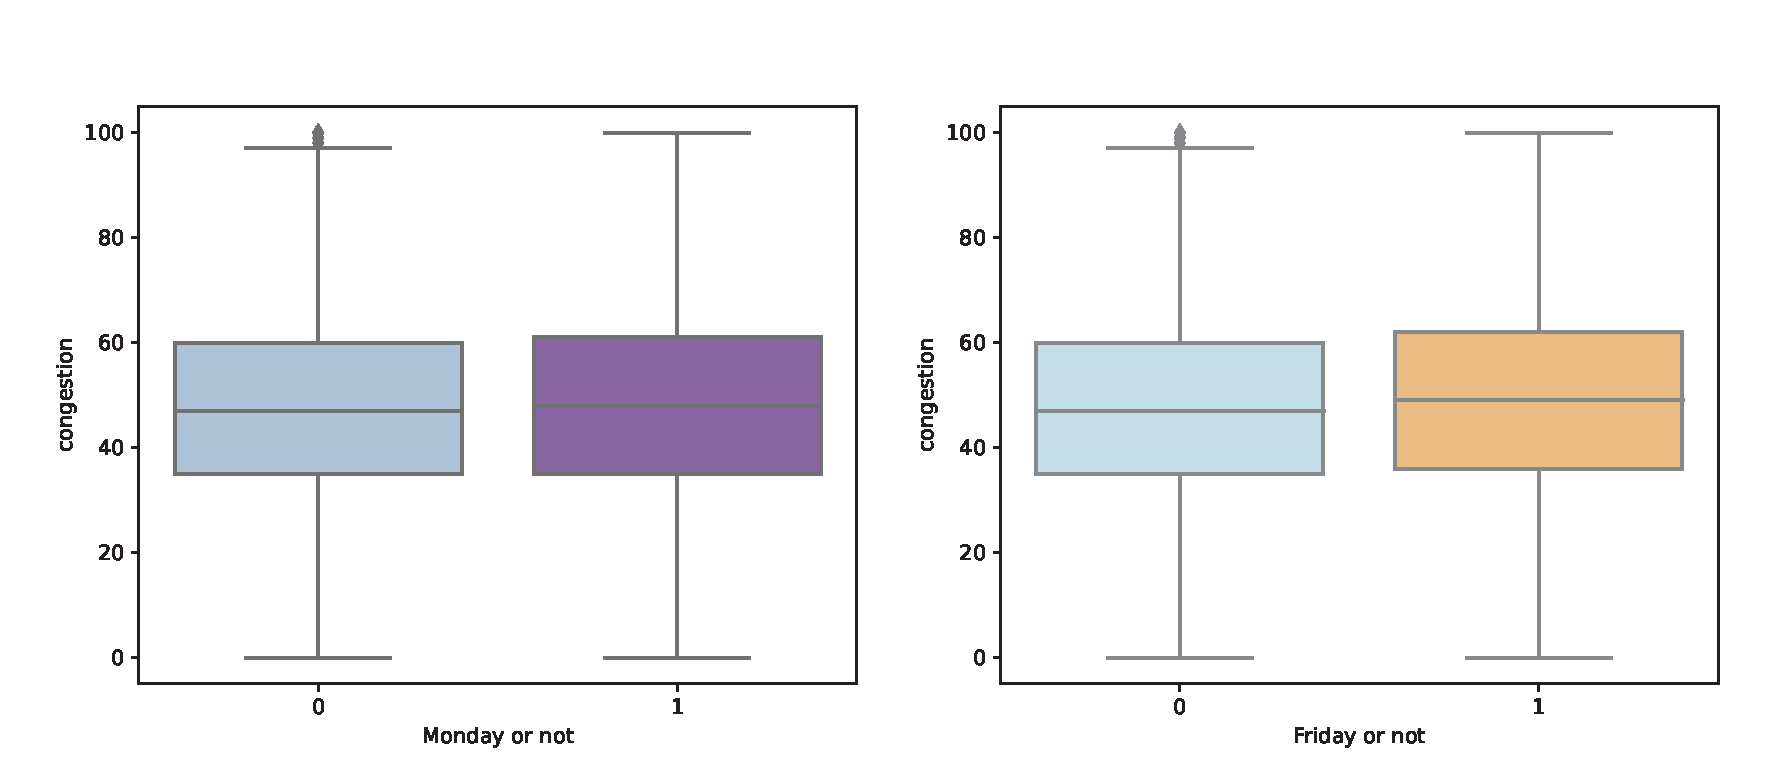
\includegraphics[width=10cm]{figure/is_weekend.eps}
	\centering
	\caption{\DIFaddFL{Congestion in special day or not}}
	\label{special}
	\end{figure}
\end{center}
\DIFaddend 

\DIFdelbegin \DIFdel{Test citation~\mbox{%DIFAUXCMD
\cite{BL12J01}}\hskip0pt%DIFAUXCMD
. 
}%DIFDELCMD < \begin{JournalOnly}
%DIFDELCMD < %%%
\DIFdel{and~\mbox{%DIFAUXCMD
\citep{BJL11J01} }\hskip0pt%DIFAUXCMD
or~\mbox{%DIFAUXCMD
\citet{BJL11J01}}\hskip0pt%DIFAUXCMD
.
}%DIFDELCMD < \end{JournalOnly}
%DIFDELCMD < %%%
\DIFdelend \DIFaddbegin \begin{center}
	\begin{figure}[htp]
		\setlength{\abovecaptionskip}{0.1cm} 
		\raggedleft
		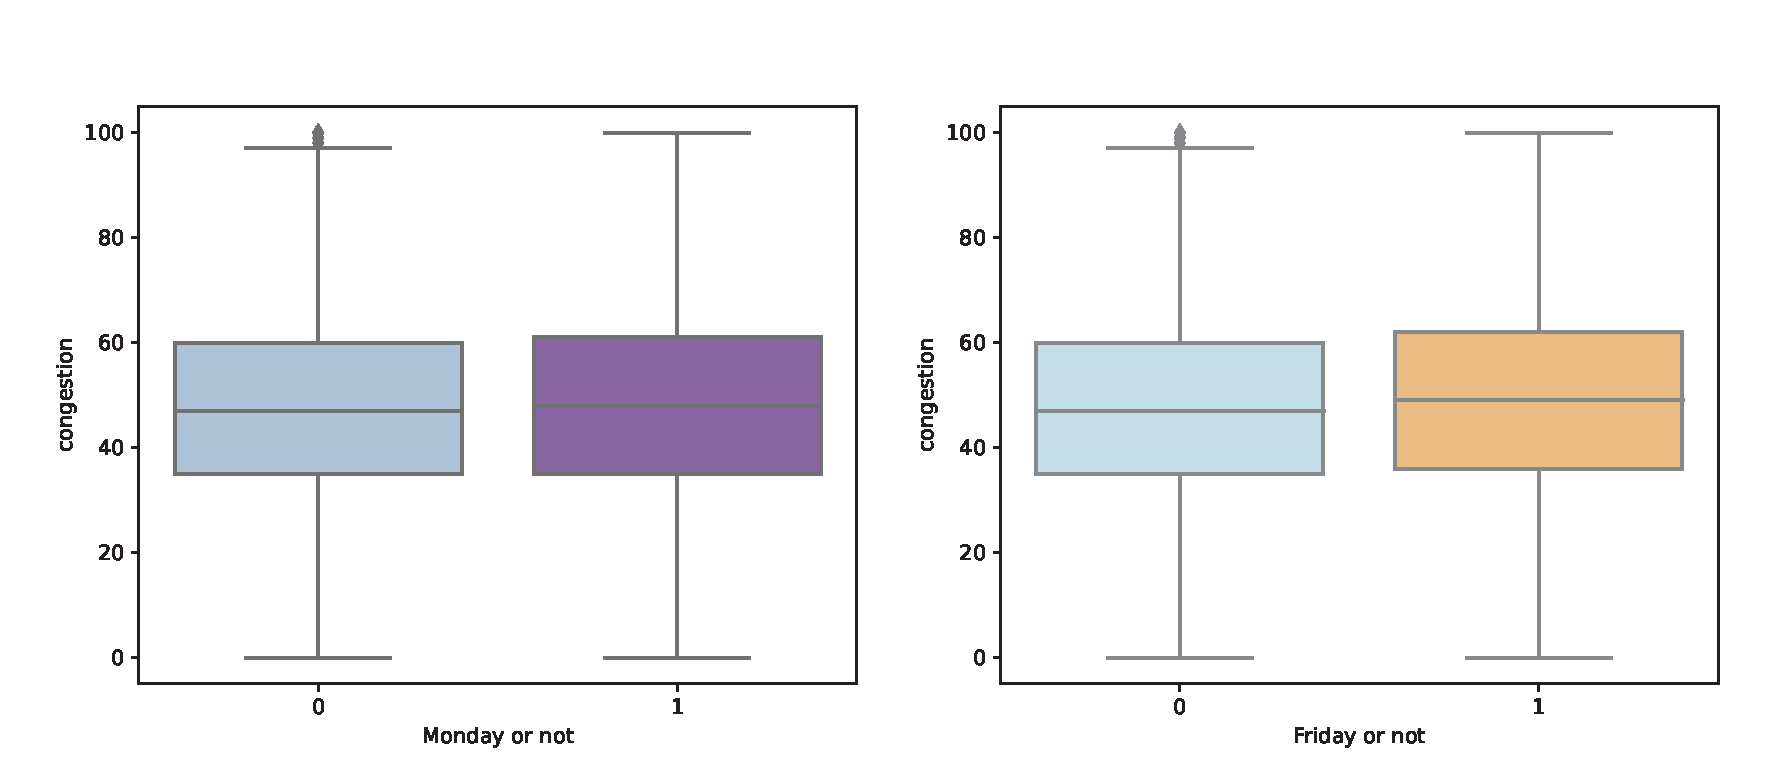
\includegraphics[width=10cm]{figure/is_weekend.eps}
		\centering
		\caption{\DIFaddFL{Congestion in special day or not}}
		\label{special}
	\end{figure}
\end{center}
\DIFaddend 

\DIFdelbegin \DIFdel{This is for ~}%DIFDELCMD < \cref{tbl:overall-experiments}%%%
\DIFdel{,}%DIFDELCMD < \todo[fancyline]{Testing.}
%DIFDELCMD < %%%
\DIFdel{and this is for~}%DIFDELCMD < \cref{sec-conclusions}%%%
\DIFdel{.
}%DIFDELCMD < \todo[noline]{A note with no line back to the text.}%%%
%DIF < 
%DIFDELCMD < \gangli{This is comment from Gang.}
%DIFDELCMD < \qwu{Response from QW}
%DIFDELCMD < %%%
\DIFdelend \DIFaddbegin \begin{center}
	\DIFaddend 

	\DIFdelbegin \DIFdel{Number:}%DIFDELCMD < \num{123}%%%
\DIFdel{.
}%DIFDELCMD < \numlist{10;30;50;70}%%%
\DIFdel{, }%DIFDELCMD < \numrange{10}{30}%%%
\DIFdel{,
}%DIFDELCMD < \SIlist{10;30;45}{\metre}%%%
\DIFdel{,
and }%DIFDELCMD < \SI{10}{\percent}
%DIFDELCMD < %%%
\DIFdelend \DIFaddbegin \begin{figure}
		\setlength{\abovecaptionskip}{0.1cm} 
		\raggedleft
		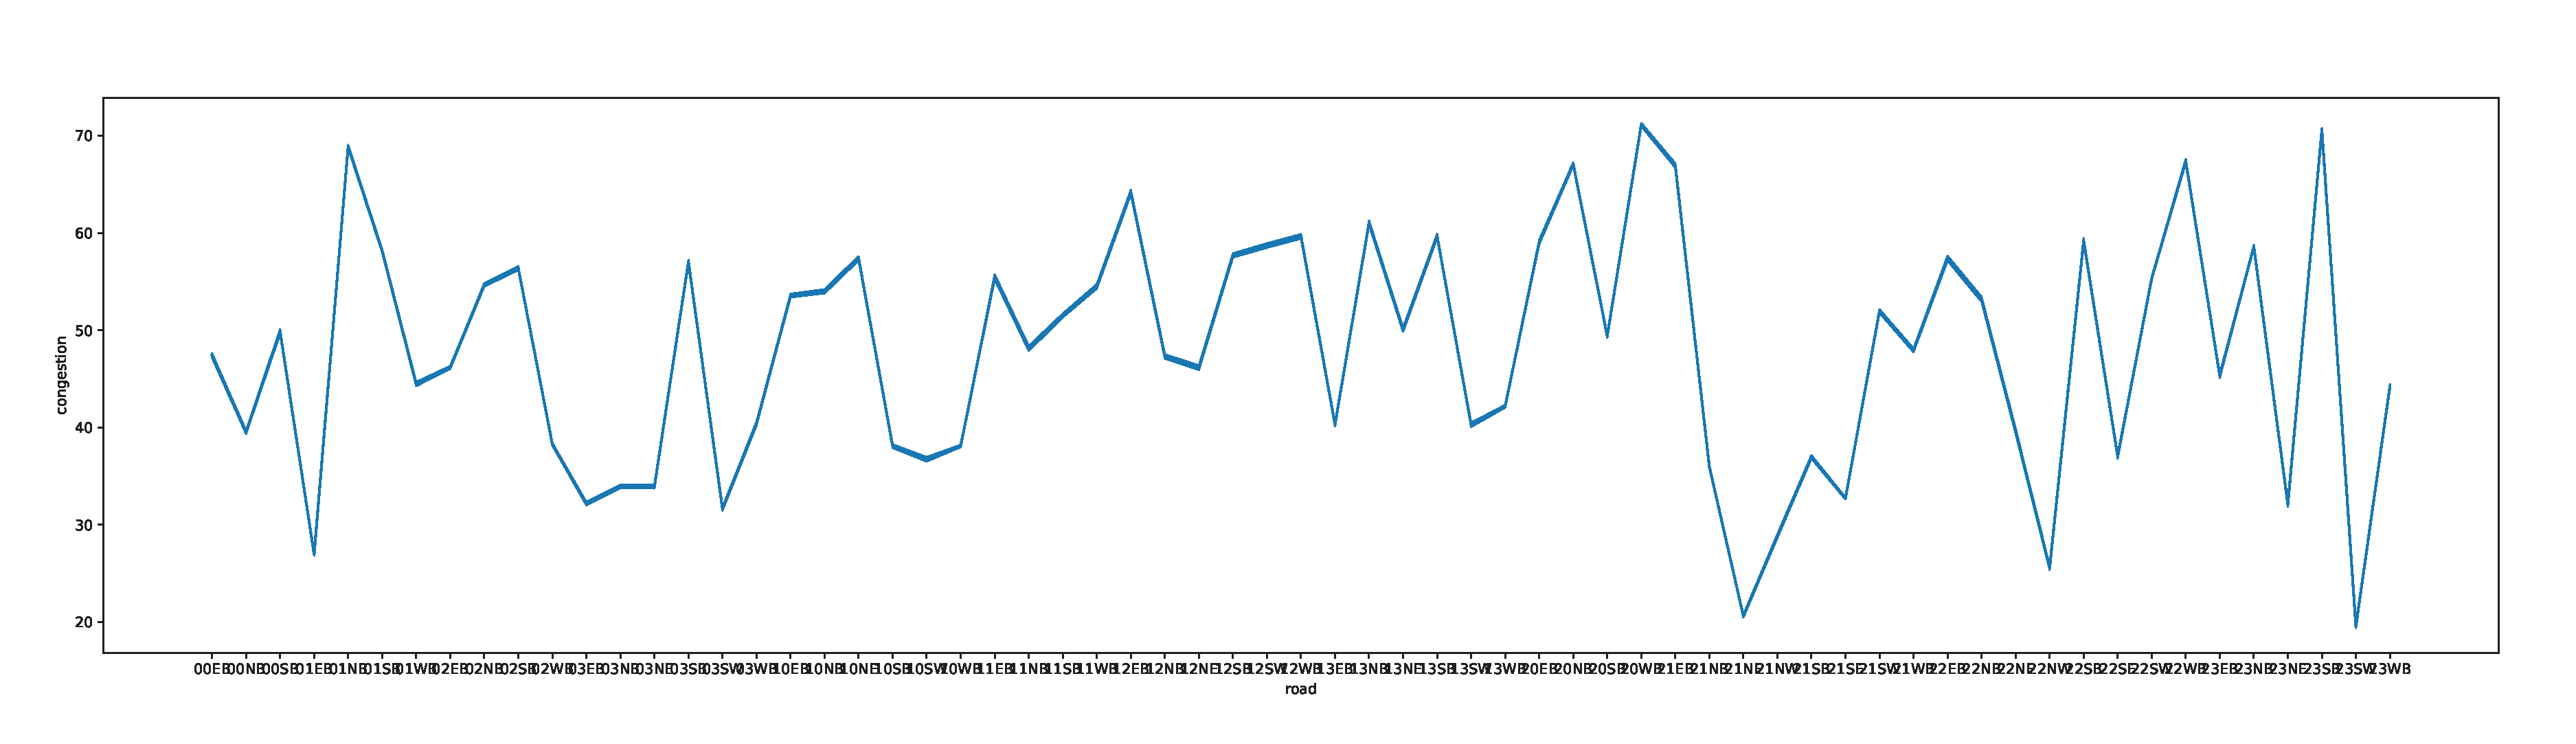
\includegraphics[width=10.0cm]{figure/road1.eps}
		\centering
		\caption{\DIFaddFL{The effect of road on congestion}}
		\label{road}
	\end{figure}
\end{center}
\DIFaddend 

\DIFdelbegin %DIFDELCMD < \missingfigure[figcolor=white]{Testing figcolor}
%DIFDELCMD < %%%
\DIFdelend \DIFaddbegin \begin{center}
	\begin{figure}
		\setlength{\abovecaptionskip}{0.1cm} 
		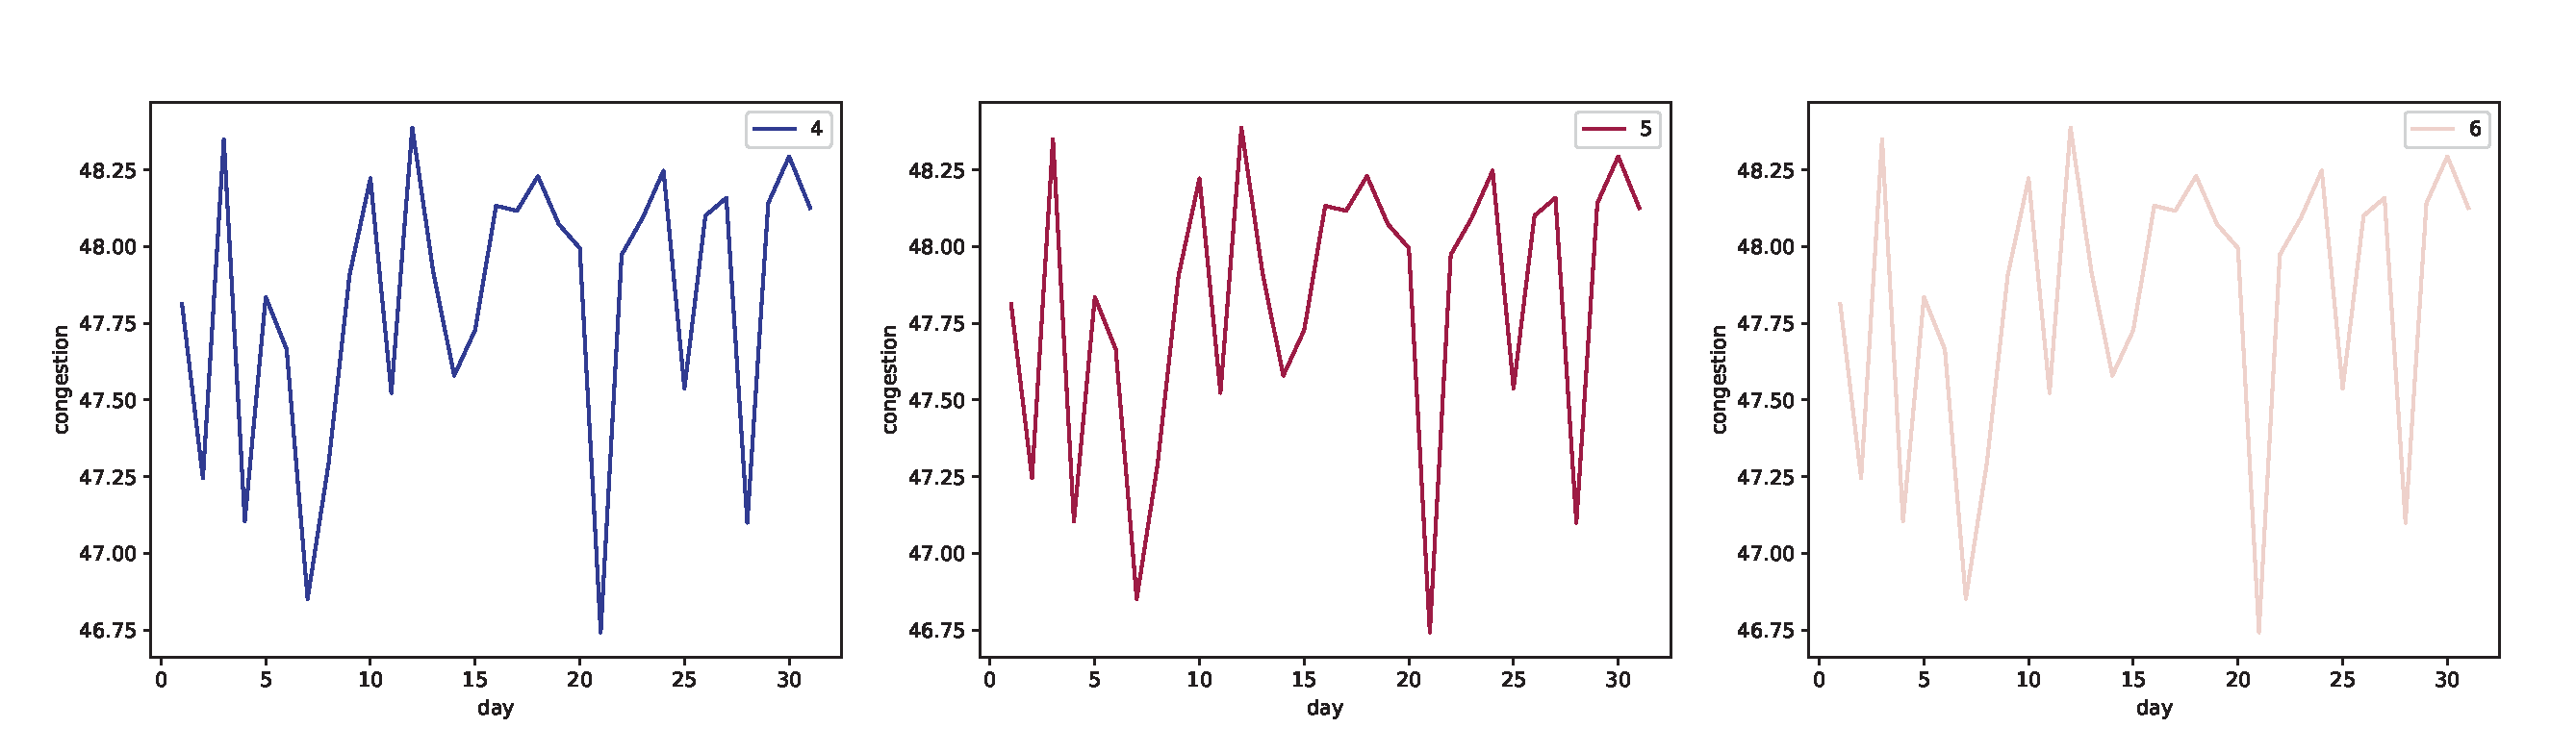
\includegraphics[width=10.0cm]{figure/day.eps}
		\caption{\DIFaddFL{The effect of day on congestion group by month}}
		\label{day}
	\end{figure}
\end{center}
\DIFaddend 

\DIFdelbegin %DIFDELCMD < \begin{ConferenceOnly}
%DIFDELCMD < %%%
\DIFdel{We have }%DIFDELCMD < \SI{10}{\hertz}%%%
\DIFdel{, }%DIFDELCMD < \si{\kilogram\metre\per\second}%%%
\DIFdel{,
the range: }%DIFDELCMD < \SIrange{10}{100}{\hertz}%%%
\DIFdel{.
$\nicefrac[]{1}{2}$.
}\DIFdelend \DIFaddbegin \begin{figure}
		\setlength{\abovecaptionskip}{0.1cm} 
		\raggedleft
		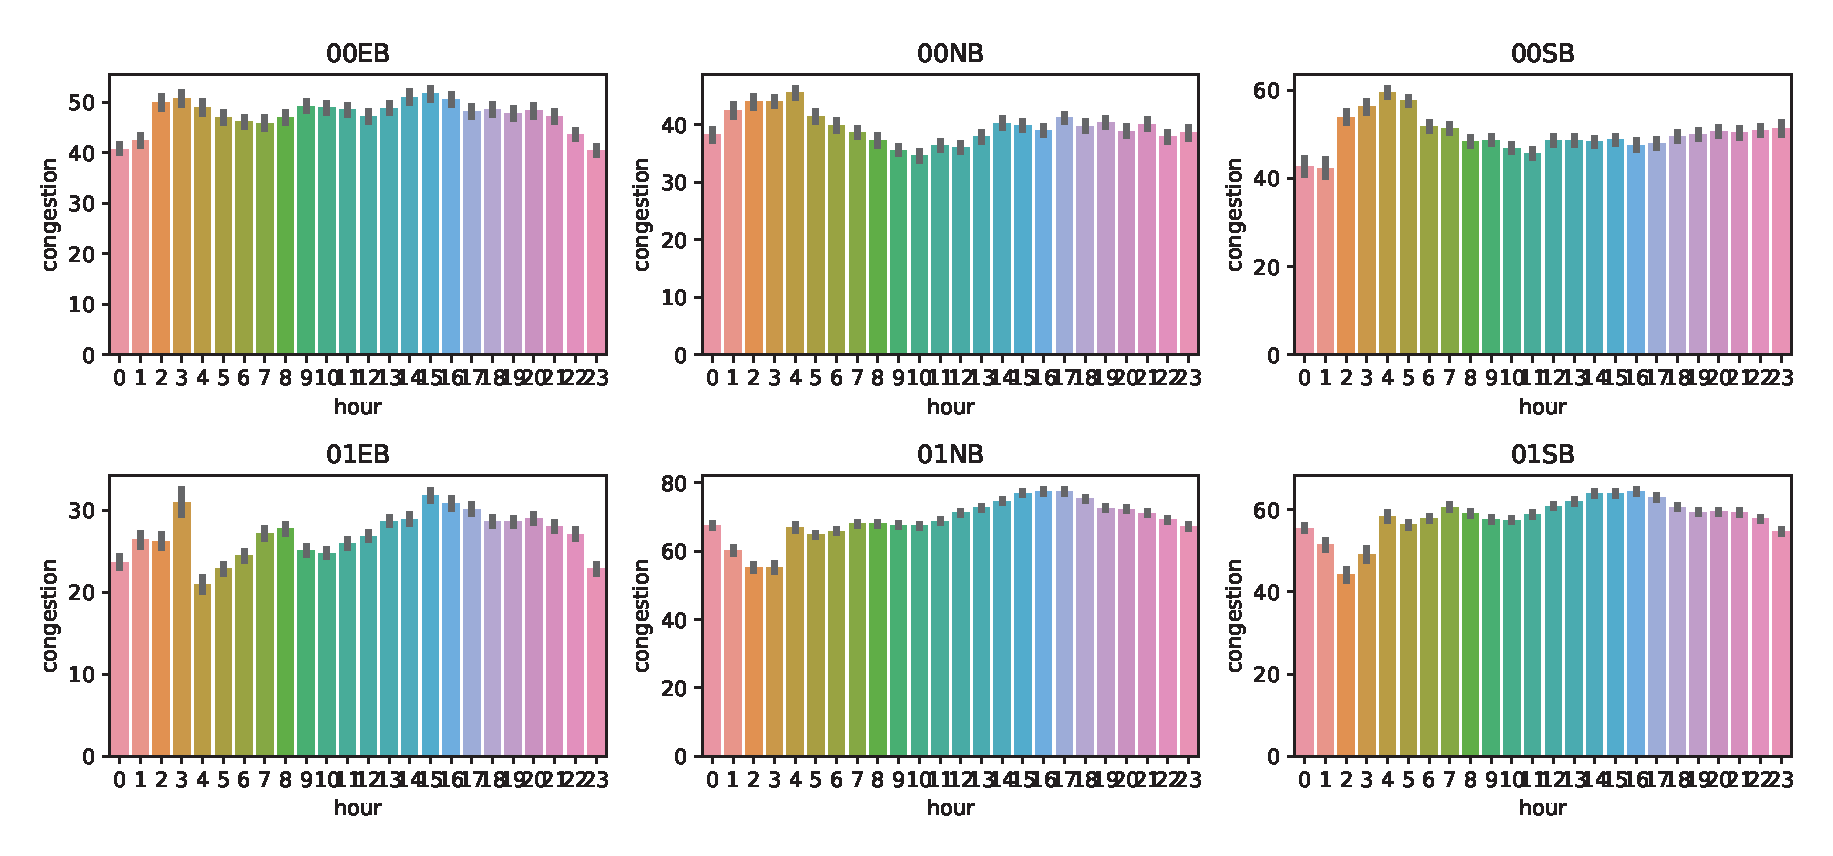
\includegraphics[width=10.0cm]{figure/road.eps}
		\centering
		\caption{\DIFaddFL{The effect of hour on congestion group by road}}
		\label{group by road}
\end{figure}
\DIFaddend 

\DIFdelbegin %DIFDELCMD < \missingfigure{Make a sketch of the structure of a trebuchet.}
%DIFDELCMD < %%%
\DIFdelend \DIFaddbegin \begin{figure}
	\DIFaddendFL 

		\DIFdelbeginFL %DIFDELCMD < \end{ConferenceOnly}
%DIFDELCMD < %%%
\DIFdelendFL \DIFaddbeginFL \setlength{\abovecaptionskip}{0.1cm} 
		\raggedleft
		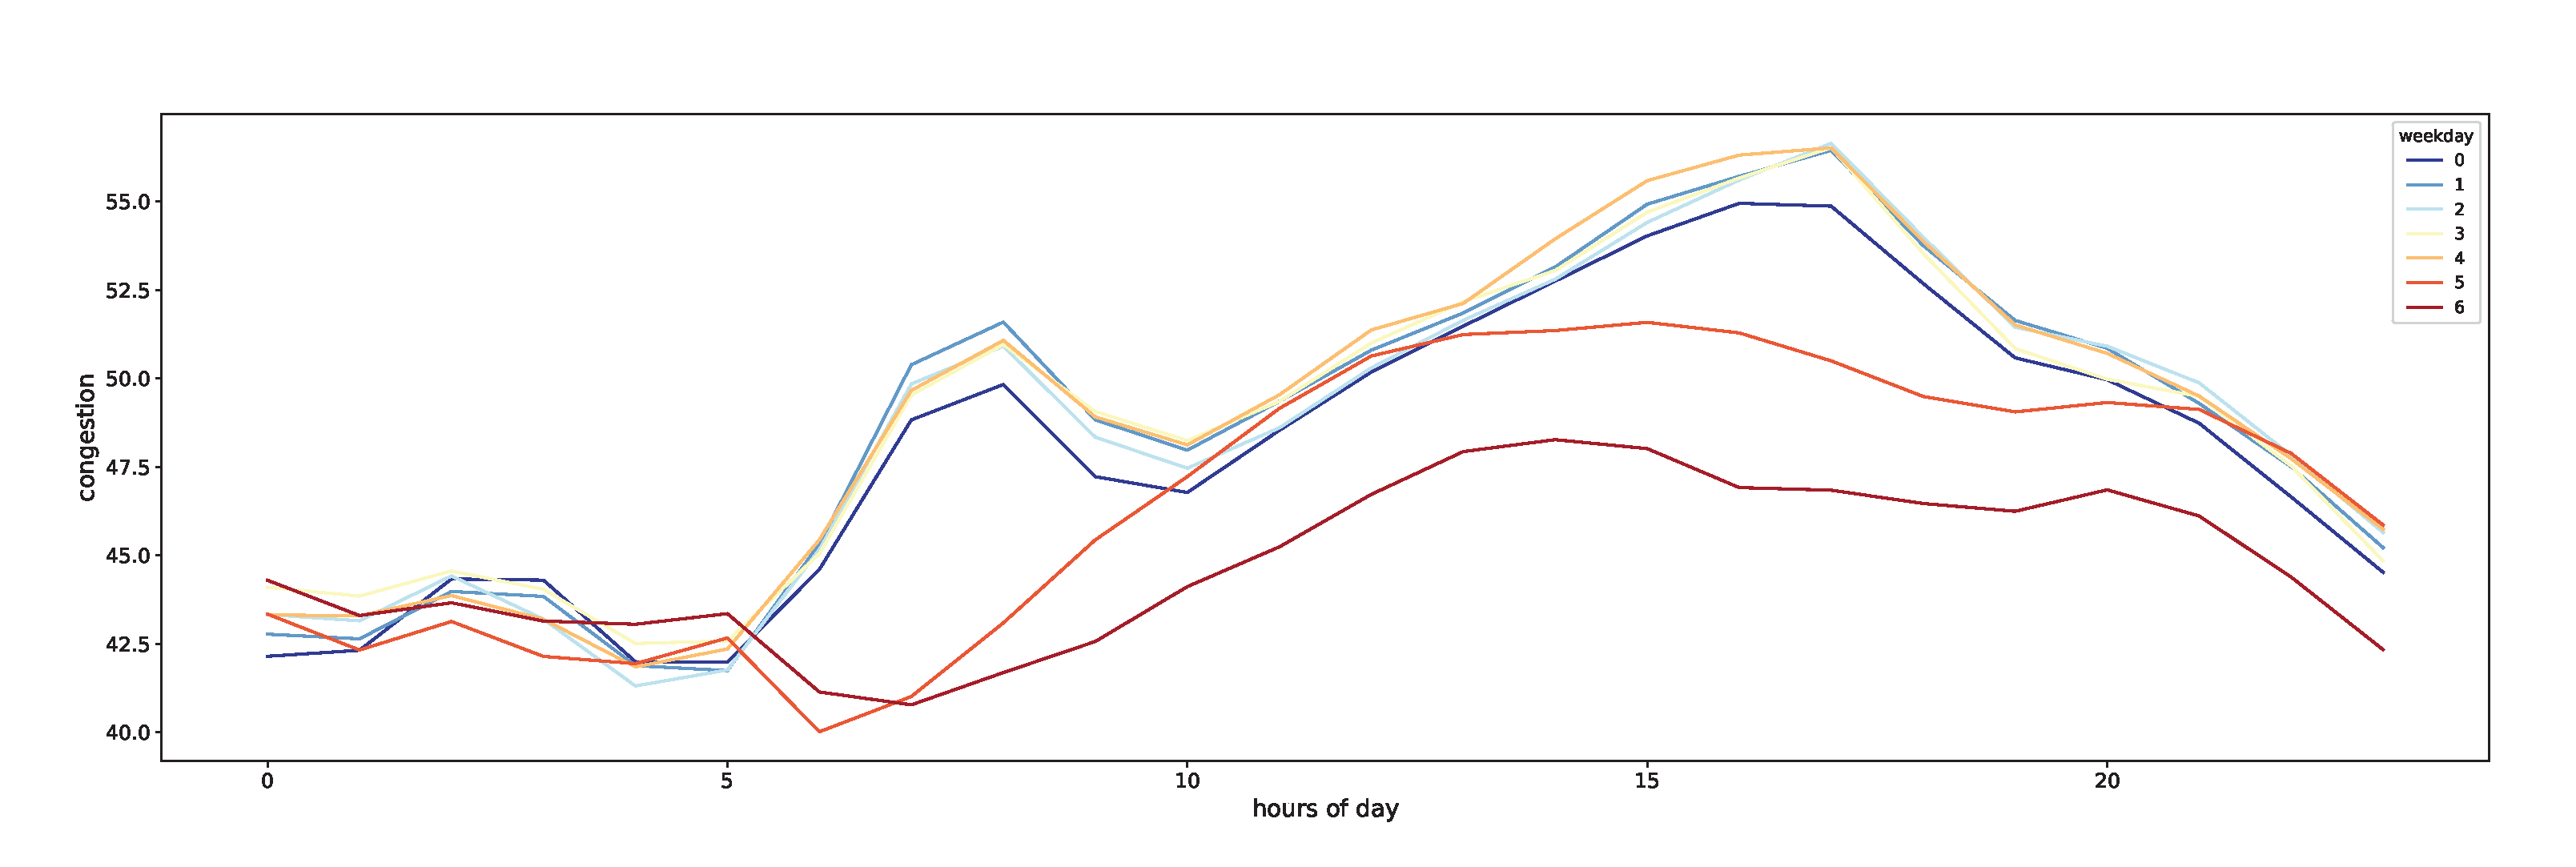
\includegraphics[width=10.0cm]{figure/hour.eps}
		\centering
		\caption{\DIFaddFL{The effect of weekday on congestion group by hour}}
		\label{group by hour}
\end{figure}
\DIFaddend 

\DIFdelbegin \DIFdel{For~}%DIFDELCMD < \cref{eq:test}%%%
\DIFdel{, as shown below:
}\DIFdelend \DIFaddbegin \begin{center}
	\begin{figure}
			\setlength{\abovecaptionskip}{0.1cm} 
			\raggedleft
			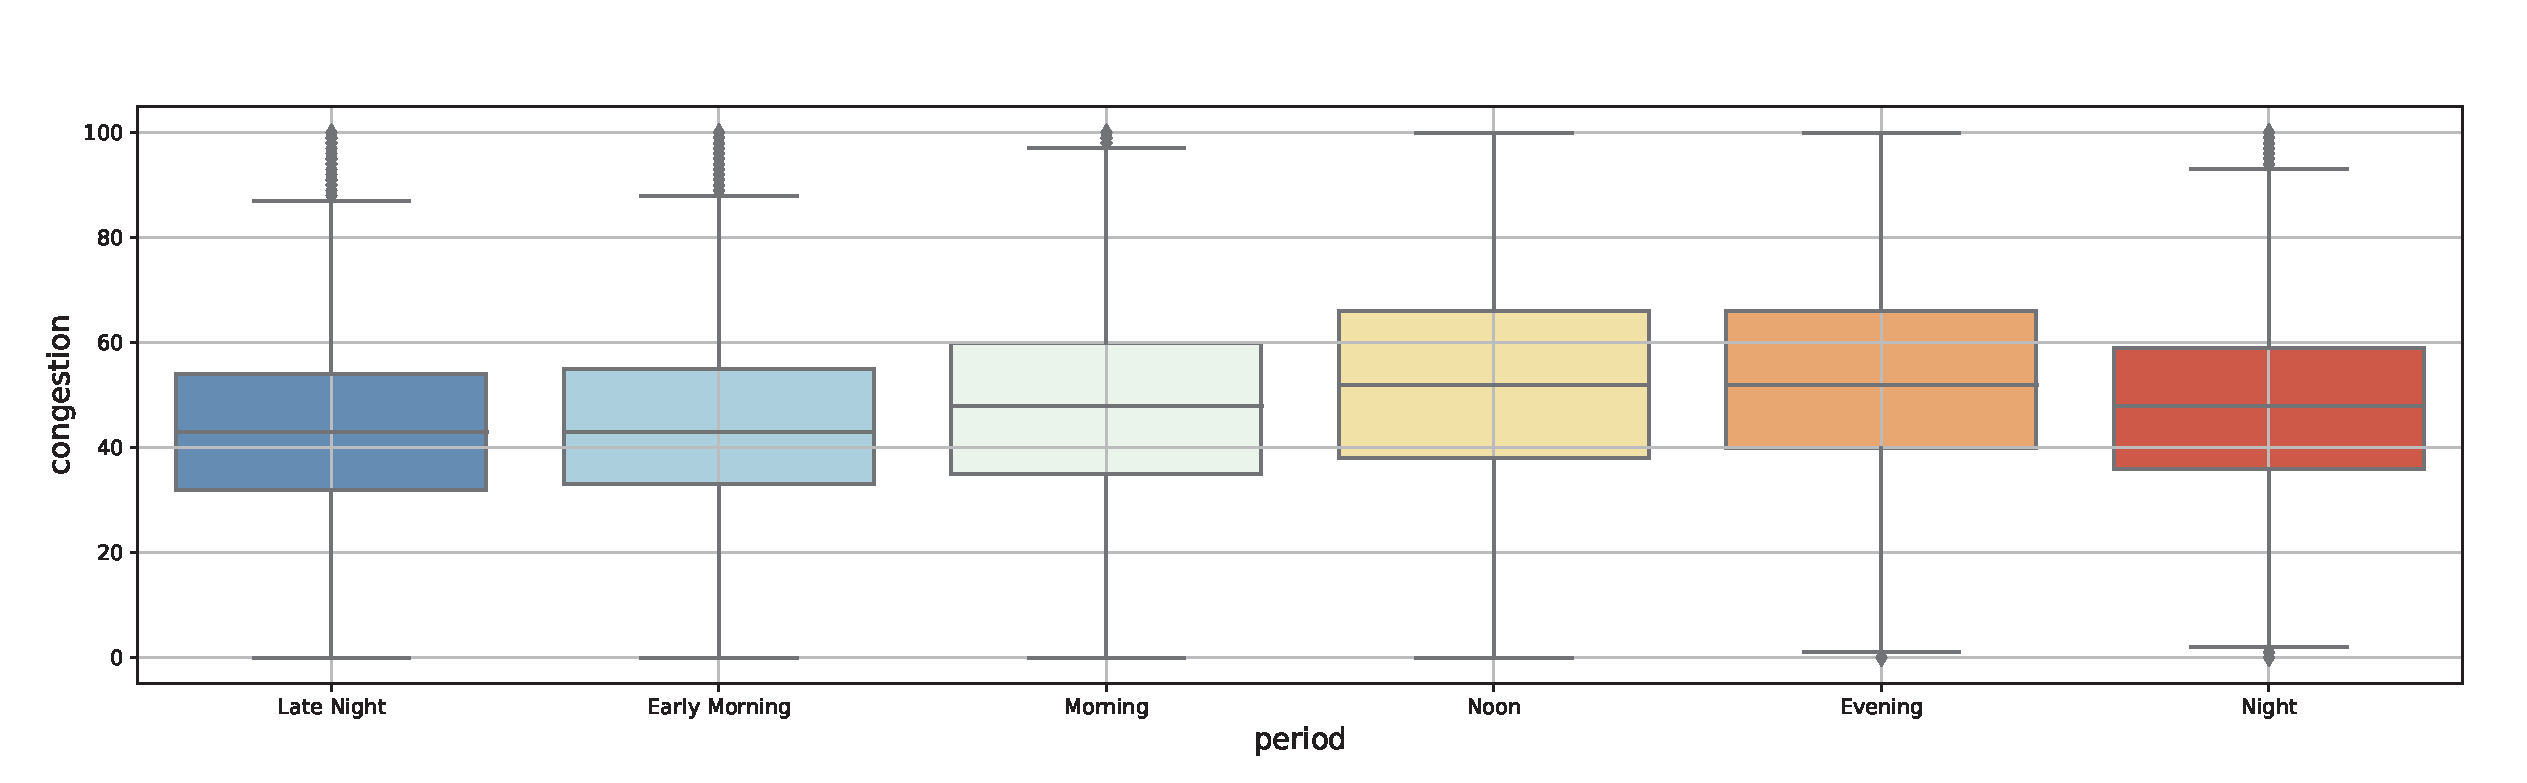
\includegraphics[width=10.0cm]{figure/period.eps}
			\centering
			\caption{\DIFaddFL{The effect of period on congestion}}
			\label{period}
	\end{figure}
\end{center}
\DIFaddend 

\DIFdelbegin \begin{displaymath}\DIFdel{%DIFDELCMD < \label{eq:test}%%%
a = b \times \sqrt{ab}
}\end{displaymath}%DIFAUXCMD
%DIFDELCMD < 

%DIFDELCMD < \blindmathpaper
%DIFDELCMD < 

%DIFDELCMD < %%%
\section{\DIFdel{Preliminaries}} %DIFAUXCMD
\addtocounter{section}{-1}%DIFAUXCMD
%DIFDELCMD < \label{sec-preliminaries}
%DIFDELCMD < 

%DIFDELCMD < \blindtext
%DIFDELCMD < 

%DIFDELCMD < \gliMarker  %%%
%DIF < TODO: GLi Here
%DIFDELCMD < 

%DIFDELCMD < %%%
\section{\DIFdel{Method}} %DIFAUXCMD
\addtocounter{section}{-1}%DIFAUXCMD
%DIFDELCMD < \label{sec-method}
%DIFDELCMD < 

%DIFDELCMD < \blindtext
%DIFDELCMD < \blindlist{itemize}[3]
%DIFDELCMD < \blinditemize
%DIFDELCMD < \blindenumerate
%DIFDELCMD < 

%DIFDELCMD < \blindmathtrue
%DIFDELCMD < \blindmathfalse
%DIFDELCMD < \blinddescription
%DIFDELCMD < 

%DIFDELCMD < \qwuMarker %%%
%DIF < TODO: QWu Here
%DIFDELCMD < 

%DIFDELCMD < %%%
\section{\DIFdel{Experiment and Analysis}} %DIFAUXCMD
\addtocounter{section}{-1}%DIFAUXCMD
\DIFdelend \DIFaddbegin \section{\DIFadd{Model Train and Evaluation}} \DIFaddend \label{sec-experiment}
\DIFaddbegin \DIFadd{Before training the model, we carried out the following steps:}\par
\begin{enumerate}
	\item \DIFadd{Divide the training and validation sets using sklearn's library.
	}\item \DIFadd{Process the non-integer data from the training set, validation set and test set
}\end{enumerate}\par
\DIFadd{In this paper, a lightgbm model is used to train to predict congestion in the US metropolitan area with the following parameter settings:}\par
\DIFadd{'objective' : 'regression'}\par
\DIFadd{'metric': 'mae'}\par
\DIFadd{'learning_rate': 0.25}\par
\DIFadd{'num_iteration': 200}\par
\DIFadd{'num_leaves':250}\par
\DIFadd{'device':'gpu'}\par
\DIFadd{After setting up the model parameters, we encapsulated the data into the format required by lightgbm for training.}\par
\DIFadd{As the training was completed, we extracted the following features.(figure 10)}\par
\begin{figure}[h]
	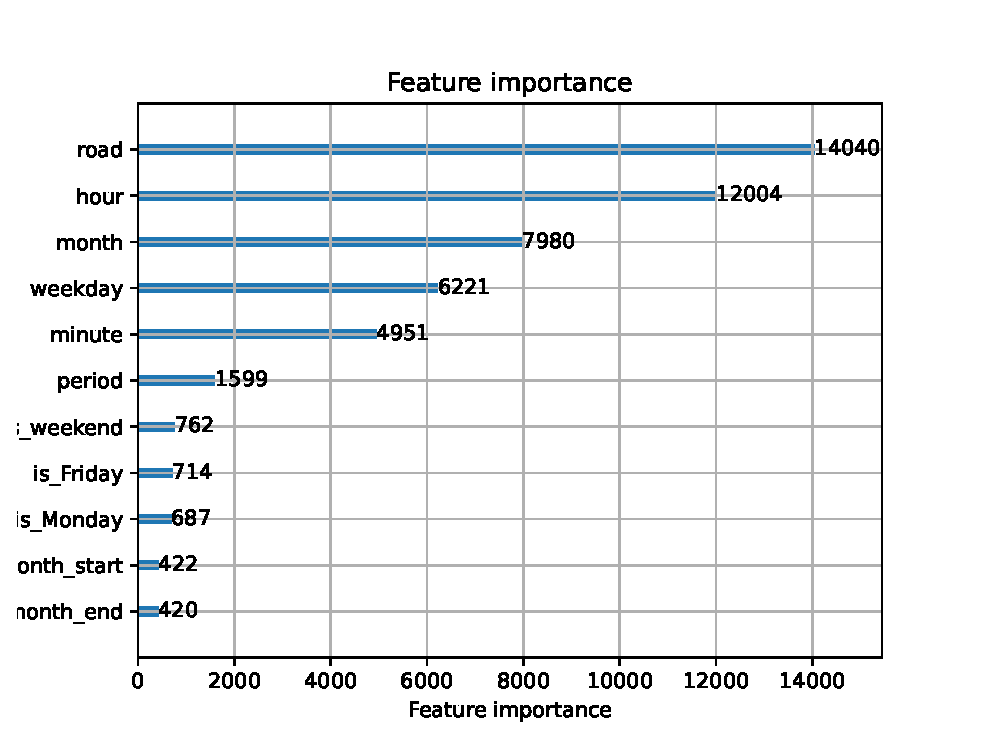
\includegraphics[width=8cm]{figure/feature_importance.eps}
	\caption{\DIFaddFL{Feature Importance}}
\end{figure}\par
\DIFadd{In the evaluation phase of the model, we evaluated the model using the regression model evaluation metrics. The evaluation indicators are listed in the table 3 below:}\par
\begin{table}[htb]
	\setlength{\abovecaptionskip}{0pt}
	\setlength{\belowcaptionskip}{10pt}
	\centering
	\caption{\DIFaddFL{Model evaluation indexes}}
	\DIFaddendFL 

	\DIFdelbeginFL %DIFDELCMD < \begin{table}  %%%
\DIFdelendFL \DIFaddbeginFL \begin{tabular}{ c | c  }
		\toprule
		\DIFaddFL{Index    }&  \DIFaddFL{Eexplication }\\
		\midrule
		\DIFaddFL{explained_variance_score     }&  \makecell{Explain the variance score of \\the regression model. }   \\
		\DIFaddFL{mean_absolute_error		  }&  \makecell{Assess the proximity of the predicted results to\\the real data set.} \\
		\DIFaddFL{Mean squared error				  }&  \makecell{Calculate the mean value of the square sum of the errors\\ of the corresponding sample points of the \\fitting data and the original data} \\
		\DIFaddFL{r2_score				  			 }&   \makecell{Judge the fitting degree of prediction model and real data} \\
		\bottomrule
	\end{tabular}
\end{table}
\DIFadd{Three of these indicators were used for the assessment,the results of the assessment are as follows:}\par
\begin{table}[htb]
	\setlength{\belowcaptionskip}{10pt}
	\caption{\DIFaddFL{The Evaluation results}}
	\begin{tabular}{c|c}
		\hline
		\DIFaddFL{Index }& \DIFaddFL{Result  }\\
		\hline
		\DIFaddFL{explained_variance_score   }& \DIFaddFL{0.7277243544483329    }\\
		\DIFaddFL{mean_absolute_error}&  \DIFaddFL{6.167491947603395 }\\
		\DIFaddFL{r2_score }& \DIFaddFL{0.7277251135484366  }\\
		\hline
	\end{tabular}
\end{table}\par
\DIFadd{From Table 4, it can be seen that both explained_variance_score and r2_score are 0.73, so the model is well trained without optimization.
}

\section{\DIFadd{Result}} \label{sec-conclusions}
\DIFadd{Based on the data from the test set, some of the test results are shown in the table 5 below:}\par
\begin{table}[htb]
	\setlength{\abovecaptionskip}{10pt}
	\setlength{\belowcaptionskip}{15pt}
	\DIFaddendFL \centering
	\caption{\DIFdelbeginFL \DIFdelFL{Precision Comparison on Event Detection Methods}\DIFdelendFL \DIFaddbeginFL \DIFaddFL{The prediction results}\DIFaddendFL }
	\DIFdelbeginFL %DIFDELCMD < \label{tbl:overall-experiments}
%DIFDELCMD <   \begin{tabular}{cccc}
%DIFDELCMD < \toprule
%DIFDELCMD <     %%%
%DIF <  after \\: \hline or \cline{col1-col2} \cline{col3-col4} ...
    \DIFdelendFL \DIFaddbeginFL 

	\begin{tabular}{p{2.5cm}p{2.5cm}p{2.5cm}p{2.5cm}}
		\hline
		\DIFaddFL{Row_id }\DIFaddendFL & \DIFdelbeginFL \DIFdelFL{OR Event Detection }\DIFdelendFL \DIFaddbeginFL \DIFaddFL{Congestion  }\DIFaddendFL &  \DIFdelbeginFL \DIFdelFL{AC Event Detection }\DIFdelendFL \DIFaddbeginFL \DIFaddFL{Row_id }\DIFaddendFL & \DIFdelbeginFL \DIFdelFL{TC Event Detection }\DIFdelendFL \DIFaddbeginFL \DIFaddFL{Congestion }\DIFaddendFL \\
		\DIFdelbeginFL %DIFDELCMD < \midrule
%DIFDELCMD <     %%%
\DIFdelFL{precision }\DIFdelendFL \DIFaddbeginFL 
		\\hline
		\DIFaddFL{848835 }\DIFaddendFL & \DIFdelbeginFL \DIFdelFL{0.83 }\DIFdelendFL \DIFaddbeginFL \DIFaddFL{47 }\DIFaddendFL & \DIFdelbeginFL \DIFdelFL{0.69 }\DIFdelendFL \DIFaddbeginFL \DIFaddFL{848836 }\DIFaddendFL & \DIFdelbeginFL \DIFdelFL{0.46 }\DIFdelendFL \DIFaddbeginFL \DIFaddFL{33}\DIFaddendFL \\
		\DIFdelbeginFL \DIFdelFL{recall }\DIFdelendFL \DIFaddbeginFL \DIFaddFL{848837 }\DIFaddendFL & \DIFdelbeginFL \DIFdelFL{0.68 }\DIFdelendFL \DIFaddbeginFL \DIFaddFL{39 }\DIFaddendFL & \DIFdelbeginFL \DIFdelFL{0.48 }\DIFdelendFL \DIFaddbeginFL \DIFaddFL{848838 }\DIFaddendFL & \DIFdelbeginFL \DIFdelFL{0.36 }\DIFdelendFL \DIFaddbeginFL \DIFaddFL{54}\DIFaddendFL \\
		\DIFdelbeginFL \DIFdelFL{F-score }\DIFdelendFL \DIFaddbeginFL \DIFaddFL{848839 }\DIFaddendFL & \DIFdelbeginFL \DIFdelFL{0.747 }\DIFdelendFL \DIFaddbeginFL \DIFaddFL{64 }\DIFaddendFL & \DIFdelbeginFL \DIFdelFL{0.57 }\DIFdelendFL \DIFaddbeginFL \DIFaddFL{848840 }\DIFaddendFL & \DIFdelbeginFL \DIFdelFL{0.4 }\DIFdelendFL \DIFaddbeginFL \DIFaddFL{23}\DIFaddendFL \\
		\DIFdelbeginFL %DIFDELCMD < \bottomrule
%DIFDELCMD < %%%
\DIFdelendFL \DIFaddbeginFL \DIFaddFL{848841 }& \DIFaddFL{28 }& \DIFaddFL{848842 }& \DIFaddFL{70}\\
		\DIFaddFL{848843 }& \DIFaddFL{25 }& \DIFaddFL{848844 }& \DIFaddFL{47}\\
		\DIFaddFL{848845 }& \DIFaddFL{46 }& \DIFaddFL{848846 }& \DIFaddFL{25}\\
		\DIFaddFL{848847 }& \DIFaddFL{69 }& \DIFaddFL{848848 }& \DIFaddFL{60}\\
		\hline
	\DIFaddendFL \end{tabular}
\end{table}
\DIFdelbegin %DIFDELCMD < 

%DIFDELCMD < %%%
\section{\DIFdel{Conclusions}} %DIFAUXCMD
\addtocounter{section}{-1}%DIFAUXCMD
%DIFDELCMD < \label{sec-conclusions}
%DIFDELCMD < 

%DIFDELCMD < \blindtext
%DIFDELCMD < 

%DIFDELCMD < %%%
\section*{\DIFdel{Acknowledgement}}
%DIFAUXCMD
%DIFDELCMD < 

%DIFDELCMD < \lipsum[1]
%DIFDELCMD < 

%DIFDELCMD < %%%
\DIFdel{The authors would like to thank \ldots
}\DIFdelend 




